%class
	\documentclass{beamer}

%template
	\usetheme{HannoverSalman}
	\setbeamertemplate{navigation symbols}{}
	%\setbeamertemplate{footline}{\centering{\insertframenumber/\insertpresentationendpage}}
	%\setbeamertemplate{footline}{\hspace*{.5cm}\scriptsize{\hfill\insertframenumber\hspace*{.5cm}}} 


%packages
	\usepackage{amsmath, amssymb, graphicx,cancel}
	\usepackage[absolute,overlay]{textpos}
	\usepackage{subfigure}
	\usepackage{caption}\captionsetup{labelformat=empty,labelsep=none}
	\usepackage{geometry}
	\geometry{verbose}
	\usepackage{color}
	\usepackage{xmpmulti}
	\usepackage[3D]{movie15}
	\usepackage{hyperref}
%	\usepackage{bookmark}
	\usepackage[open,openlevel=4,atend]{bookmark}
	%\bookmarksetup{color=blue}
	\usepackage{multirow}
	\usepackage[style=numeric,defernumbers, authoryear]{biblatex}
	%\usepackage[square,sort]{natbib}
	%\usepackage{fancyhdr}%\pagestyle{fancy} 

	
	\hypersetup{bookmarksdepth = 4}


%citations files
	\bibliography{MyCitations}

%logoCSIPCPL
    \setlength{\TPHorizModule}{1mm}
    \setlength{\TPVertModule}{1mm}
    \newcommand{\logoCSIPCPL}
    {
    	\begin{textblock}{1}(100,2) %(100,85)  for bottom
    		
\includegraphics[width=1.5cm]{figs/logo_CSIP}
    	\end{textblock}
    	
	\begin{textblock}{1}(117,1) %(117,85)  for bottom
    		
\includegraphics[width=1.0cm]{figs/logo_CPL}
    	\end{textblock} 
    }

%logo evolution
    \newcommand{\logoEvolution}
    {    	
	\begin{textblock}{1}(110,1) %(117,85)  for bottom
    		\includegraphics[width=0.65in]{figs/logo_evolution.pdf}
    	\end{textblock} 
    }

%logo Qualcomm
    \newcommand{\logoQualcomm}
    {
    	\begin{textblock}{1}(110,2) %(100,85)  for bottom
    		\includegraphics[width=1.5cm]{figs/logo_qualcomm.jpg}
    	\end{textblock}
    }
%logo Qualcomm (long)
    \newcommand{\logoQualcommllong}
    {
    	\begin{textblock}{1}(0,0) 
    		\includegraphics[width=1.25in]{figs/logo_qualcomm_long.jpg}
    	\end{textblock}
    }

%logo Tech Tower
    \newcommand{\logoTechTower}
    {
    	\begin{textblock}{1}(0,0) 
    		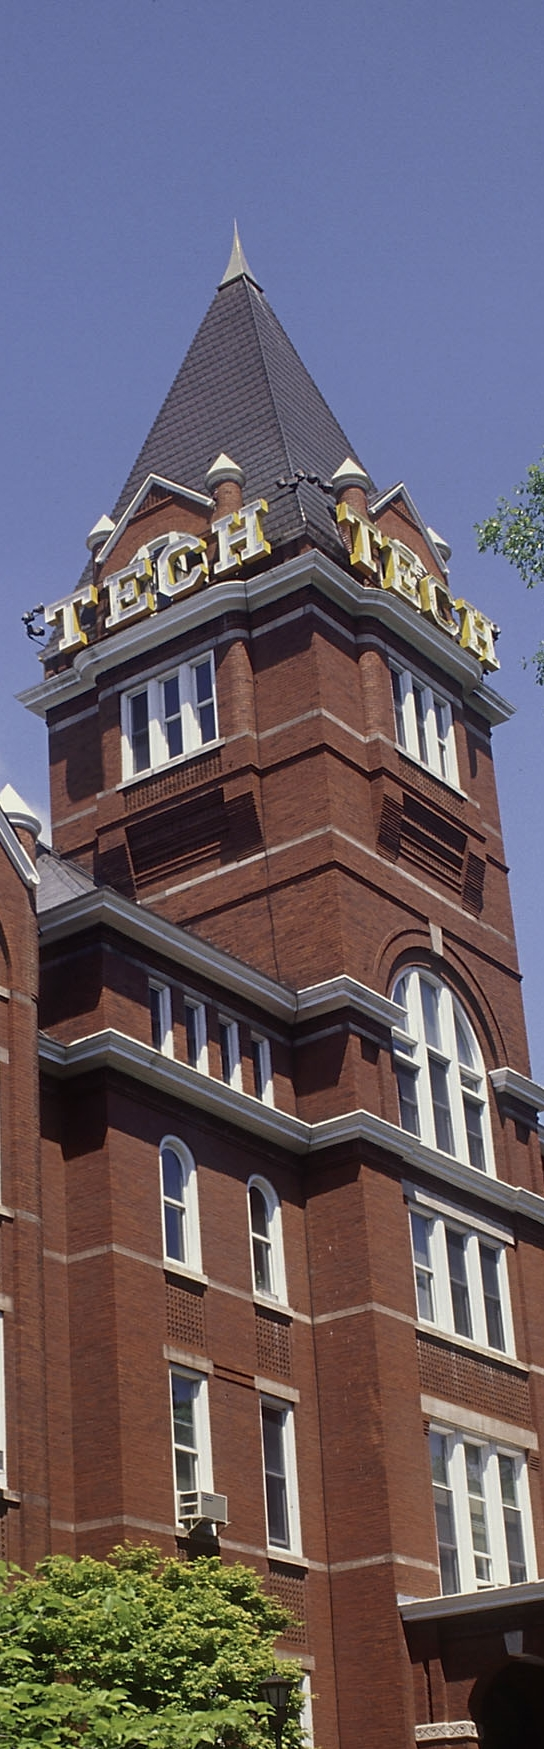
\includegraphics[width=1.25in]{figs/logo_TechTower.jpg}
    	\end{textblock}
    }

%logo tree
    \newcommand{\logoTree}
    {
    	\begin{textblock}{1}(0,0) 
    		\includegraphics[width=1.25in]{figs/logo_tree.jpg}
    	\end{textblock}
    }
%page numbers
    \newcommand{\mypagenum}
    {
    	\begin{textblock}{1}(1,94) 
		{\tiny \color[rgb]{0.2,0.2,1}\insertframenumber} %\insertframenumber,\insertpresentationendpage, \inserttotalframenumber
    	\end{textblock}
    }
%my footnote citation
	\newcommand{\myFootnoteCitation}[2]
	{
		\footnote{\tiny \citeauthor{#1}, \emph{#2}, \citeyear{#1}.}  %\citeauthor{#1}, \citetitle{#1}, #2 \citeyear{#1}.
	}
%my refer to citation
	\newcommand{\mycite}[1]
	{
		\emph{\citeauthor{#1} (\citeyear{#1})}
	}
%my footnote website citation
	\newcommand{\myFootnoteWebsiteCitation}[1]
	{
		\footnote{\tiny \citeauthor{#1}}
	}

\let\thefootnote\relax\footnotetext{Footnotetext without footnote mark}


%section underline
%\newcommand{\tmpsection}[1]{}
%\let\tmpsection=\section
%\renewcommand{\section}[1]{\tmpsection{\underline{#1}}}



%commands
	\newcommand{\likelihood}{p(Z_k| x_k) }						%likelihood
	\newcommand{\prior}{p(x_k)  } 								%prior
	\newcommand{\posterior} {p(x_k| Z_k)}						%posterior
	\newcommand{\prediction} {p(x_k| Z_{k-1})}					%prediction
	\newcommand{\update} {p(x_k|Z_k)}							%update
	\newcommand{\observations} {p(Z_k)}						%observations
	\newcommand{\prevobservations} {p(Z_{k-1})}				%previous observations
	\newcommand{\dxpk} {dx_{k-1}}							%dx_{k-1}
	\newcommand{\ChapKolm}{\int{p(x_k| x_{k-1})p(x_{k-1}|Z_{k-1})} \dxpk} %Chapman Kolmogorov

	%algorithm specific: JPDAF
	\newcommand{\likelihoodJPDAF}{p(Z_k| \chi, m, Z_{k-1}) }		%1. likelihood
	\newcommand{\priorJPDAF}{p(\chi|m, Z^{k-1}} 				%2. prior	
	\newcommand{\observationsJPDAF} {p(Z_k}					%3. observations
	\newcommand{\posteriorJPDAF} {p(\chi| Z_k)}					%4. posterior

%environments
	\newenvironment{changemargin}[2]
	{
	  	\begin{list}{}
		{
			\setlength{\topsep}{0pt}%
			\setlength{\leftmargin}{#1}%
			\setlength{\rightmargin}{#2}%
			\setlength{\listparindent}{\parindent}%
			\setlength{\itemindent}{\parindent}%
			\setlength{\parsep}{\parskip}%
		}
	  	\item[]
		}
		{\end{list}
	}
%figures

%colors
\definecolor{darkgreen}{rgb}{0,0.5,0}

%personal details
	\author{Salman Aslam}
	\institute{Advisor, Dr Christopher Barnes (ECE)\\Co-advisor, Dr Aaron Bobick (CoC)\\Georgia Institute of Technology}
	\date{}

\begin{document}
%####################################################################################################
\title{Visual Tracking \\ (Multi-view subspace)}
%####################################################################################################
\begin{frame}[plain]\logoTechTower
	\titlepage
\end{frame}

\begin{frame}
\frametitle{Outline}
\logoCSIPCPL\logoTechTower
	\setcounter{tocdepth}{1}	
	\tableofcontents
\end{frame}

%#######################################################################
\section{INTRODUCTION}
%#######################################################################
\begin{frame}
\frametitle{Introduction}
\framesubtitle{}
\logoCSIPCPL\mypagenum
\end{frame}

%#######################################################################
\section{PRIOR WORK}
%#######################################################################
%=================================
\subsection{\ \ \ \ 1990: networks for learning}
%=================================
\begin{frame}
\frametitle{Prior work: networks for learning}
\framesubtitle{overview}
\mypagenum
	{\color{blue}  \href{http://users.ece.gatech.edu/~msalman/papers/1990 JNL, Networks for Approximation and Learning (Poggio).pdf}{read paper}}
\myFootnoteCitation{1990_JNL_NetworkLearning_Poggio}{Proc. IEEE}
\end{frame}


\begin{frame}
\frametitle{Prior work: networks for learning}
\framesubtitle{figures}
\mypagenum
	\begin{figure}
		\includegraphics[height=0.75\textheight]{figs/TrackingPapers_SubspaceTracking_1990_Poggio_fig1.jpg}
	\end{figure}
\myFootnoteCitation{1990_JNL_NetworkLearning_Poggio}{Proc. IEEE}
\end{frame}


\begin{frame}
\frametitle{Prior work: networks for learning}
\framesubtitle{figures (cont.)}
\mypagenum
	\begin{figure}
		\includegraphics[height=0.75\textheight]{figs/TrackingPapers_SubspaceTracking_1990_Poggio_fig2.jpg}
	\end{figure}
\myFootnoteCitation{1990_JNL_NetworkLearning_Poggio}{Proc. IEEE}
\end{frame}


%=================================
\subsection{\ \ \ \ 1991: eigenfaces}
%=================================
\begin{frame}
\frametitle{Prior work: eigenfaces}
\framesubtitle{overview}
\mypagenum
	{\color{blue}  \href{http://users.ece.gatech.edu/~msalman/papers/1991 CNF, Face recognition using eigenfaces (Turk).pdf}{read paper}}
\myFootnoteCitation{1991_CNF_Eigenfaces_Turk}{CVPR}
\end{frame}




\begin{frame}
\frametitle{Prior work: eigenfaces}
\framesubtitle{figures}
\mypagenum
	\begin{figure}
		\includegraphics[height=0.75\textheight]{figs/TrackingPapers_SubspaceTracking_1991_Turk_fig1.jpg}
	\end{figure}
\myFootnoteCitation{1991_CNF_Eigenfaces_Turk}{CVPR}
\end{frame}


\begin{frame}
\frametitle{Prior work: eigenfaces}
\framesubtitle{figures (cont.)}
\mypagenum
	\begin{figure}
		\includegraphics[width=1.0\textwidth]{figs/TrackingPapers_SubspaceTracking_1991_Turk_fig2.jpg}
	\end{figure}
\myFootnoteCitation{1991_CNF_Eigenfaces_Turk}{CVPR}
\end{frame}


\begin{frame}
\frametitle{Prior work: eigenfaces}
\framesubtitle{figures (cont.)}
\mypagenum
	\begin{figure}
		\includegraphics[height=0.75\textheight]{figs/TrackingPapers_SubspaceTracking_1991_Turk_fig3.jpg}
	\end{figure}
\myFootnoteCitation{1991_CNF_Eigenfaces_Turk}{CVPR}
\end{frame}



\begin{frame}
\frametitle{Prior work: eigenfaces}
\framesubtitle{figures (cont.)}
\mypagenum
	\begin{figure}
		\includegraphics[height=0.75\textheight]{figs/TrackingPapers_SubspaceTracking_1991_Turk_fig4_5.jpg}
	\end{figure}
\myFootnoteCitation{1991_CNF_Eigenfaces_Turk}{CVPR}
\end{frame}


\begin{frame}
\frametitle{Prior work: eigenfaces}
\framesubtitle{figures (cont.)}
\mypagenum
	\begin{figure}
		\includegraphics[width=1.0\textwidth]{figs/TrackingPapers_SubspaceTracking_1991_Turk_fig6.jpg}
	\end{figure}
\myFootnoteCitation{1991_CNF_Eigenfaces_Turk}{CVPR}
\end{frame}


\begin{frame}
\frametitle{Prior work: eigenfaces}
\framesubtitle{figures (cont.)}
\mypagenum
	\begin{figure}
		\includegraphics[height=0.75\textheight]{figs/TrackingPapers_SubspaceTracking_1991_Turk_fig7.jpg}
	\end{figure}
\myFootnoteCitation{1991_CNF_Eigenfaces_Turk}{CVPR}
\end{frame}


%=================================
\subsection{\ \ \ \ 1995: 3D image manifolds}
%=================================
\begin{frame}
\frametitle{Prior work: Murase et al.)}
\framesubtitle{overview}
\mypagenum
	{\color{blue}  \href{http://users.ece.gatech.edu/~msalman/papers/1995 JNL, Visual learning and recognition of 3-d objects from appearance (Murase).pdf}{read paper}}
\myFootnoteCitation{1995_JNL_ImgManifolds_Murase}{IJCV}
\end{frame}



\begin{frame}
\frametitle{Prior work: Murase et al.)}
\framesubtitle{comparison}
\mypagenum
	\begin{itemize}
		\item previous representations in computer vision
			\begin{itemize}
				\item object geometry
			\end{itemize} 
		\item this paper
			\begin{itemize}
				\item object appearance
			\end{itemize} 
		\item i.e. matching appearance rather than shape
	\end{itemize}
\myFootnoteCitation{1995_JNL_ImgManifolds_Murase}{IJCV}
\end{frame}



\begin{frame}
\frametitle{Prior work (1995: 3D image manifolds)}
\framesubtitle{figures}
\mypagenum
	\begin{figure}
		\includegraphics[width=1.0\textwidth]{figs/TrackingPapers_SubspaceTracking_1995_Murase_fig1.jpg}
	\end{figure}
\myFootnoteCitation{1995_JNL_ImgManifolds_Murase}{IJCV}
\end{frame}


\begin{frame}
\frametitle{Prior work (1995: 3D image manifolds)}
\framesubtitle{figures (cont.)}
\mypagenum
	\begin{figure}
		\includegraphics[width=1.0\textwidth]{figs/TrackingPapers_SubspaceTracking_1995_Murase_fig2.jpg}
	\end{figure}
\myFootnoteCitation{1995_JNL_ImgManifolds_Murase}{IJCV}
\end{frame}



\begin{frame}
\frametitle{Prior work (1995: 3D image manifolds)}
\framesubtitle{figures (cont.)}
\mypagenum
	\begin{figure}
		\includegraphics[height=0.75\textheight]{figs/TrackingPapers_SubspaceTracking_1995_Murase_fig3.jpg}
	\end{figure}
\myFootnoteCitation{1995_JNL_ImgManifolds_Murase}{IJCV}
\end{frame}



\begin{frame}
\frametitle{Prior work (1995: 3D image manifolds)}
\framesubtitle{figures (cont.)}
\mypagenum
	\begin{figure}
		\includegraphics[height=0.75\textheight]{figs/TrackingPapers_SubspaceTracking_1995_Murase_fig4.jpg}
	\end{figure}
\myFootnoteCitation{1995_JNL_ImgManifolds_Murase}{IJCV}
\end{frame}



\begin{frame}
\frametitle{Prior work (1995: 3D image manifolds)}
\framesubtitle{figures (cont.)}
\mypagenum
	\begin{figure}
		\includegraphics[width=1.0\textwidth]{figs/TrackingPapers_SubspaceTracking_1995_Murase_fig5.jpg}
	\end{figure}
\myFootnoteCitation{1995_JNL_ImgManifolds_Murase}{IJCV}
\end{frame}


\begin{frame}
\frametitle{Prior work (1995: 3D image manifolds)}
\framesubtitle{figures (cont.)}
\mypagenum
	\begin{figure}
		\includegraphics[height=0.75\textheight]{figs/TrackingPapers_SubspaceTracking_1995_Murase_fig6.jpg}
	\end{figure}
\myFootnoteCitation{1995_JNL_ImgManifolds_Murase}{IJCV}
\end{frame}



\begin{frame}
\frametitle{Prior work (1995: 3D image manifolds)}
\framesubtitle{figures (cont.)}
\mypagenum
	\begin{figure}
		\includegraphics[height=0.75\textheight]{figs/TrackingPapers_SubspaceTracking_1995_Murase_fig7.jpg}
	\end{figure}
\myFootnoteCitation{1995_JNL_ImgManifolds_Murase}{IJCV}
\end{frame}



\begin{frame}
\frametitle{Prior work (1995: Murase et al.)}
\framesubtitle{figures (cont.)}
\mypagenum
	\begin{figure}
		\includegraphics[width=1.0\textwidth]{figs/TrackingPapers_SubspaceTracking_1995_Murase_fig8.jpg}
	\end{figure}
\myFootnoteCitation{1995_JNL_ImgManifolds_Murase}{IJCV}
\end{frame}



\begin{frame}
\frametitle{Prior work (1995: 3D image manifolds)}
\framesubtitle{figures (cont.)}
\mypagenum
	\begin{figure}
		\includegraphics[width=1.0\textwidth]{figs/TrackingPapers_SubspaceTracking_1995_Murase_fig9.jpg}
	\end{figure}
\myFootnoteCitation{1995_JNL_ImgManifolds_Murase}{IJCV}
\end{frame}


\begin{frame}
\frametitle{Prior work (1995: 3D image manifolds)}
\framesubtitle{figures (cont.)}
\mypagenum
	\begin{figure}
		\includegraphics[height=0.75\textheight]{figs/TrackingPapers_SubspaceTracking_1995_Murase_fig10.jpg}
	\end{figure}
\myFootnoteCitation{1995_JNL_ImgManifolds_Murase}{IJCV}
\end{frame}




%=================================
\subsection{\ \ \ \ 1996: eigentracking}
%=================================

\begin{frame}
\frametitle{Prior work: eigentracking}
\framesubtitle{1. overview}
\logoCSIPCPL\mypagenum
	{\color{blue}  \href{http://users.ece.gatech.edu/~msalman/papers/1998 JNL, EigenTracking_ robust matching and tracking of articulated objects using a view-based representation (Black, Jepson, IJCV, 810).pdf}{read paper}}
\myFootnoteCitation{1998_JNL_Eigentracking_Black}{IJCV}
\end{frame}




\begin{frame}
\frametitle{Prior work: eigentracking}
\framesubtitle{1. overview}
\logoCSIPCPL\mypagenum
	\begin{figure}
		\includegraphics[width=1.0\textwidth]{tables/TrackingPapers_SubspaceTracking_1998_Black.pdf}
	\end{figure}
\myFootnoteCitation{1998_JNL_Eigentracking_Black}{IJCV}
\end{frame}



\begin{frame}
\frametitle{Prior work: eigentracking}
\framesubtitle{2. summary}
\logoCSIPCPL\mypagenum
	First appeared in ECCV 1996.  Here, we present the 1998 journal version:\\
	\begin{itemize}
		\item eigenspace tracking			
		\item input image is incrementally warped towards
eigenspace
	\end{itemize}
\myFootnoteCitation{1998_JNL_Eigentracking_Black}{IJCV}
\end{frame}


\begin{frame}
\frametitle{Prior work: eigentracking}
\framesubtitle{3. comparison}
\logoCSIPCPL\mypagenum		
	\begin{itemize}
		\item previous work was mostly on eigenspace representation for recognition, this paper first for eigentracking
	\end{itemize}
\myFootnoteCitation{1998_JNL_Eigentracking_Black}{IJCV}
\end{frame}



\begin{frame}
\frametitle{Prior work: eigentracking}
\framesubtitle{4. contributions}
\logoCSIPCPL\mypagenum
	\begin{itemize}
		\item overcome problems of the least squares approach in eigenspace methods
		\item small set of canonical views and then parameterized transformation, (eg affine) between image and eigenspace
		\item eigentracking: refine transformation between eigenspace and image
	\end{itemize}
\myFootnoteCitation{1998_JNL_Eigentracking_Black}{IJCV}
\end{frame}


\begin{frame}
\frametitle{Prior work: eigentracking}
\framesubtitle{5. methodology}
\logoCSIPCPL\mypagenum
\myFootnoteCitation{1998_JNL_Eigentracking_Black}{IJCV}
\end{frame}


\begin{frame}
\frametitle{Prior work: eigentracking}
\framesubtitle{6. computational issues}
\logoCSIPCPL\mypagenum
\myFootnoteCitation{1998_JNL_Eigentracking_Black}{IJCV}
\end{frame}


\begin{frame}
\frametitle{Prior work: eigentracking}
\framesubtitle{7. general points}
\logoCSIPCPL\mypagenum
\myFootnoteCitation{1998_JNL_Eigentracking_Black}{IJCV}
\end{frame}



\begin{frame}
\frametitle{Prior work: eigentracking}
\framesubtitle{8. limitations}
\logoCSIPCPL\mypagenum
\myFootnoteCitation{1998_JNL_Eigentracking_Black}{IJCV}
\end{frame}



\begin{frame}
\frametitle{Prior work: eigentracking}
\framesubtitle{figures}
\logoCSIPCPL\mypagenum
	\begin{figure}
		\includegraphics[width=1.0\textwidth]{figs/TrackingPapers_SubspaceTracking_1998_Black_fig1.jpg}
	\end{figure}
\myFootnoteCitation{1998_JNL_Eigentracking_Black}{IJCV}
\end{frame}



\begin{frame}
\frametitle{Prior work: eigentracking}
\framesubtitle{figures (cont.)}
\logoCSIPCPL\mypagenum
	\begin{figure}
		\includegraphics[width=1.0\textwidth]{figs/TrackingPapers_SubspaceTracking_1998_Black_fig2_3.jpg}
	\end{figure}
\myFootnoteCitation{1998_JNL_Eigentracking_Black}{IJCV}
\end{frame}



\begin{frame}
\frametitle{Prior work: eigentracking}
\framesubtitle{figures (cont.)}
\logoCSIPCPL\mypagenum
	\begin{figure}
		\includegraphics[width=1.0\textwidth]{figs/TrackingPapers_SubspaceTracking_1998_Black_fig4.jpg}
	\end{figure}
\myFootnoteCitation{1998_JNL_Eigentracking_Black}{IJCV}
\end{frame}



\begin{frame}
\frametitle{Prior work: eigentracking}
\framesubtitle{figures (cont.)}
\logoCSIPCPL\mypagenum
	\begin{figure}
		\includegraphics[width=1.0\textwidth]{figs/TrackingPapers_SubspaceTracking_1998_Black_fig5.jpg}
	\end{figure}
\myFootnoteCitation{1998_JNL_Eigentracking_Black}{IJCV}
\end{frame}




\begin{frame}
\frametitle{Prior work: eigentracking}
\framesubtitle{figures (cont.)}
\logoCSIPCPL\mypagenum
	\begin{figure}
		\includegraphics[width=1.0\textwidth]{figs/TrackingPapers_SubspaceTracking_1998_Black_fig6.jpg}
	\end{figure}
\myFootnoteCitation{1998_JNL_Eigentracking_Black}{IJCV}
\end{frame}




\begin{frame}
\frametitle{Prior work: eigentracking}
\framesubtitle{figures (cont.)}
\logoCSIPCPL\mypagenum
	\begin{figure}
		\includegraphics[width=1.0\textwidth]{figs/TrackingPapers_SubspaceTracking_1998_Black_fig7.jpg}
	\end{figure}
\myFootnoteCitation{1998_JNL_Eigentracking_Black}{IJCV}
\end{frame}



\begin{frame}
\frametitle{Prior work: eigentracking}
\framesubtitle{figures (cont.)}
\logoCSIPCPL\mypagenum
	\begin{figure}
		\includegraphics[width=1.0\textwidth]{figs/TrackingPapers_SubspaceTracking_1998_Black_fig8.jpg}
	\end{figure}
\myFootnoteCitation{1998_JNL_Eigentracking_Black}{IJCV}
\end{frame}



\begin{frame}
\frametitle{Prior work: eigentracking}
\framesubtitle{figures (cont.)}
\logoCSIPCPL\mypagenum
	\begin{figure}
		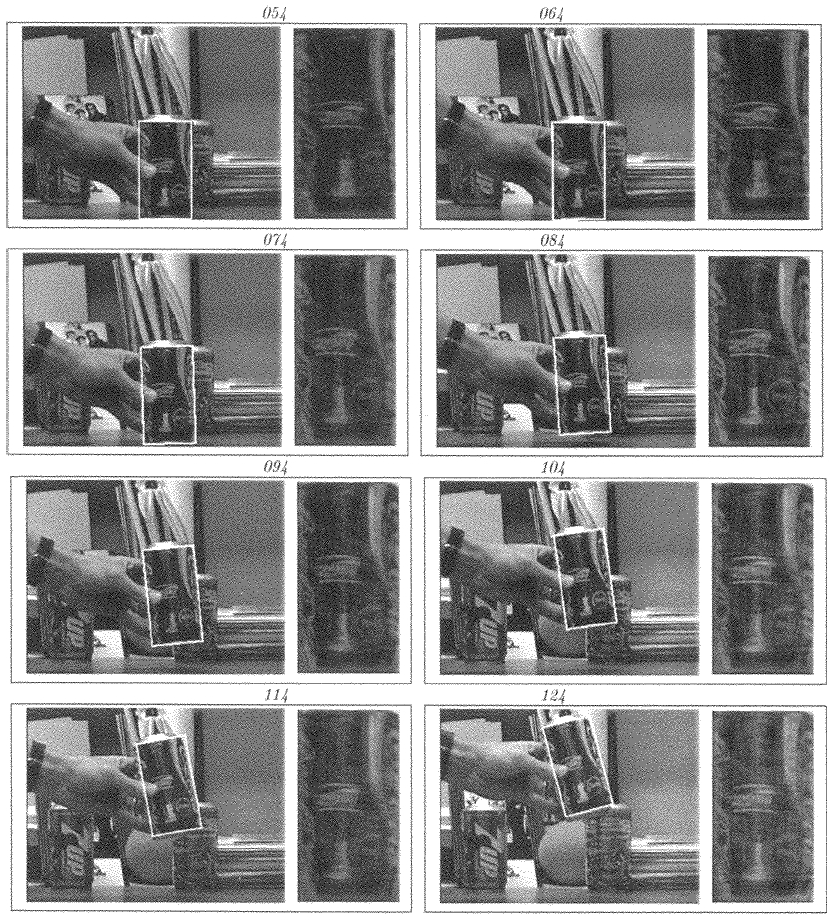
\includegraphics[height=0.75\textheight]{figs/TrackingPapers_SubspaceTracking_1998_Black_fig9.jpg}
	\end{figure}
\myFootnoteCitation{1998_JNL_Eigentracking_Black}{IJCV}
\end{frame}




\begin{frame}
\frametitle{Prior work: eigentracking}
\framesubtitle{figures (cont.)}
\logoCSIPCPL\mypagenum
	\begin{figure}
		\includegraphics[width=1.0\textwidth]{figs/TrackingPapers_SubspaceTracking_1998_Black_fig10.jpg}
	\end{figure}
\myFootnoteCitation{1998_JNL_Eigentracking_Black}{IJCV}
\end{frame}


\begin{frame}
\frametitle{Prior work: eigentracking}
\framesubtitle{figures (cont.)}
\logoCSIPCPL\mypagenum
	\begin{figure}
		\includegraphics[width=0.8\textwidth]{figs/TrackingPapers_SubspaceTracking_1998_Black_fig11.jpg}
	\end{figure}
\myFootnoteCitation{1998_JNL_Eigentracking_Black}{IJCV}
\end{frame}




\begin{frame}
\frametitle{Prior work: eigentracking}
\framesubtitle{figures (cont.)}
\logoCSIPCPL\mypagenum
	\begin{figure}
		\includegraphics[height=0.75\textheight]{figs/TrackingPapers_SubspaceTracking_1998_Black_fig12.jpg}
	\end{figure}
\myFootnoteCitation{1998_JNL_Eigentracking_Black}{IJCV}
\end{frame}




\begin{frame}
\frametitle{Prior work: eigentracking}
\framesubtitle{figures (cont.)}
\logoCSIPCPL\mypagenum
	\begin{figure}
		\includegraphics[height=0.75\textheight]{figs/TrackingPapers_SubspaceTracking_1998_Black_fig13.jpg}
	\end{figure}
\myFootnoteCitation{1998_JNL_Eigentracking_Black}{IJCV}
\end{frame}



\begin{frame}
\frametitle{Prior work: eigentracking}
\framesubtitle{figures (cont.)}
\logoCSIPCPL\mypagenum
	\begin{figure}
		\includegraphics[width=1.0\textwidth]{figs/TrackingPapers_SubspaceTracking_1998_Black_fig14_15.jpg}
	\end{figure}
\myFootnoteCitation{1998_JNL_Eigentracking_Black}{IJCV}
\end{frame}


\begin{frame}
\frametitle{Prior work: eigentracking}
\framesubtitle{figures (cont.)}
\logoCSIPCPL\mypagenum
	\begin{figure}
		\includegraphics[width=1.0\textwidth]{figs/TrackingPapers_SubspaceTracking_1998_Black_fig16.jpg}
	\end{figure}
\myFootnoteCitation{1998_JNL_Eigentracking_Black}{IJCV}
\end{frame}

%=================================
\subsection{\ \ \ \ 1997: eigen vs. fisher faces}
%=================================
\begin{frame}
\frametitle{Prior work: eigen vs fisher faces}
\framesubtitle{overview}
\mypagenum
	{\color{blue}  \href{http://users.ece.gatech.edu/~msalman/papers/1997 JNL, Eigenfaces vs. Fisherfaces_ recognition using class specific linear projection (Belhumeur).pdf}{read paper}}
\myFootnoteCitation{1997_JNL_EigenVsFisherFaces_Bel}{PAMI}
\end{frame}






\begin{frame}
\frametitle{Prior work: eigen vs fisher faces}
\framesubtitle{figures}
\mypagenum
	\begin{figure}
		\includegraphics[width=1.0\textwidth]{figs/TrackingPapers_SubspaceTracking_1997_Belhumeur_fig1.jpg}
	\end{figure}
\myFootnoteCitation{1997_JNL_EigenVsFisherFaces_Bel}{PAMI}
\end{frame}



\begin{frame}
\frametitle{Prior work: eigen vs fisher faces}
\framesubtitle{figures (cont.)}
\mypagenum
	\begin{figure}
		\includegraphics[height=0.75\textheight]{figs/TrackingPapers_SubspaceTracking_1997_Belhumeur_fig2.jpg}
	\end{figure}
\myFootnoteCitation{1997_JNL_EigenVsFisherFaces_Bel}{PAMI}
\end{frame}


\begin{frame}
\frametitle{Prior work: eigen vs fisher faces}
\framesubtitle{figures (cont.)}
\mypagenum
	\begin{figure}
		\includegraphics[width=1.0\textwidth]{figs/TrackingPapers_SubspaceTracking_1997_Belhumeur_fig3.jpg}
	\end{figure}
\myFootnoteCitation{1997_JNL_EigenVsFisherFaces_Bel}{PAMI}
\end{frame}



\begin{frame}
\frametitle{Prior work: eigen vs fisher faces}
\framesubtitle{figures (cont.)}
\mypagenum
	\begin{figure}
		\includegraphics[width=1.0\textwidth]{figs/TrackingPapers_SubspaceTracking_1997_Belhumeur_fig4.jpg}
	\end{figure}
\myFootnoteCitation{1997_JNL_EigenVsFisherFaces_Bel}{PAMI}
\end{frame}



\begin{frame}
\frametitle{Prior work: eigen vs fisher faces}
\framesubtitle{figures (cont.)}
\mypagenum
	\begin{figure}
		\includegraphics[width=1.0\textwidth]{figs/TrackingPapers_SubspaceTracking_1997_Belhumeur_fig5.jpg}
	\end{figure}
\myFootnoteCitation{1997_JNL_EigenVsFisherFaces_Bel}{PAMI}
\end{frame}



\begin{frame}
\frametitle{Prior work: eigen vs fisher faces}
\framesubtitle{figures (cont.)}
\mypagenum
	\begin{figure}
		\includegraphics[width=1.0\textwidth]{figs/TrackingPapers_SubspaceTracking_1997_Belhumeur_fig6.jpg}
	\end{figure}
\myFootnoteCitation{1997_JNL_EigenVsFisherFaces_Bel}{PAMI}
\end{frame}



\begin{frame}
\frametitle{Prior work: eigen vs fisher faces}
\framesubtitle{figures (cont.)}
\mypagenum
	\begin{figure}
		\includegraphics[width=1.0\textwidth]{figs/TrackingPapers_SubspaceTracking_1997_Belhumeur_fig7.jpg}
	\end{figure}
\myFootnoteCitation{1997_JNL_EigenVsFisherFaces_Bel}{PAMI}
\end{frame}



\begin{frame}
\frametitle{Prior work: eigen vs fisher faces}
\framesubtitle{figures (cont.)}
\mypagenum
	\begin{figure}
		\includegraphics[width=1.0\textwidth]{figs/TrackingPapers_SubspaceTracking_1997_Belhumeur_fig8.jpg}
	\end{figure}
\myFootnoteCitation{1997_JNL_EigenVsFisherFaces_Bel}{PAMI}
\end{frame}



\begin{frame}
\frametitle{Prior work: eigen vs fisher faces}
\framesubtitle{figures (cont.)}
\mypagenum
	\begin{figure}
		\includegraphics[width=1.0\textwidth]{figs/TrackingPapers_SubspaceTracking_1997_Belhumeur_fig9.jpg}
	\end{figure}
\myFootnoteCitation{1997_JNL_EigenVsFisherFaces_Bel}{PAMI}
\end{frame}



\begin{frame}
\frametitle{Prior work: eigen vs fisher faces}
\framesubtitle{figures (cont.)}
\mypagenum
	\begin{figure}
		\includegraphics[width=1.0\textwidth]{figs/TrackingPapers_SubspaceTracking_1997_Belhumeur_fig10.jpg}
	\end{figure}
\myFootnoteCitation{1997_JNL_EigenVsFisherFaces_Bel}{PAMI}
\end{frame}



\begin{frame}
\frametitle{Prior work: eigen vs fisher faces}
\framesubtitle{figures (cont.)}
\mypagenum
	\begin{figure}
		\includegraphics[width=1.0\textwidth]{figs/TrackingPapers_SubspaceTracking_1997_Belhumeur_table1.jpg}
	\end{figure}
\myFootnoteCitation{1997_JNL_EigenVsFisherFaces_Bel}{PAMI}
\end{frame}






%=================================
\subsection{\ \ \ \ 1997: eigenspace density tracking}
%=================================
\begin{frame}
\frametitle{Prior work: eigenspace density estimation}
\framesubtitle{summary}
\mypagenum
		{\color{blue}  \href{http://users.ece.gatech.edu/~msalman/papers/1997 JNL, Probabilistic visual learning for object representation (Moghaddam, Pentland, PAMI, 1163).pdf}{read paper}}
\myFootnoteCitation{1997_JNL_EigenTRK_Moghaddam}{PAMI}
\end{frame}



\begin{frame}
\frametitle{Prior work: eigenspace density estimation}
\framesubtitle{summary}
\mypagenum
	\begin{itemize}
		\item eigenspace density estimation for unsupervised visual learning
		\item estimator is based on a subspace decomposition and can be evaluated using the $M$-dimensional principal component vector
	\end{itemize}
\myFootnoteCitation{1997_JNL_EigenTRK_Moghaddam}{PAMI}
\end{frame}



\begin{frame}
\frametitle{Prior work: eigenspace density estimation}
\framesubtitle{figures}
\mypagenum
	\begin{figure}
		\includegraphics[height=0.7\textheight]{figs/TrackingPapers_SubspaceTracking_1997_Moghaddam_fig1.jpg}
	\end{figure}
\myFootnoteCitation{1997_JNL_EigenTRK_Moghaddam}{PAMI}
\end{frame}


\begin{frame}
\frametitle{Prior work: eigenspace density estimation}
\framesubtitle{figures (cont.)}
\mypagenum
	\begin{figure}
		\includegraphics[height=0.7\textheight]{figs/TrackingPapers_SubspaceTracking_1997_Moghaddam_fig2.jpg}
	\end{figure}
\myFootnoteCitation{1997_JNL_EigenTRK_Moghaddam}{PAMI}
\end{frame}


\begin{frame}
\frametitle{Prior work: eigenspace density estimation}
\framesubtitle{figures (cont.)}
\mypagenum
	\begin{figure}
		\includegraphics[width=1.0\textwidth]{figs/TrackingPapers_SubspaceTracking_1997_Moghaddam_fig3.jpg}
	\end{figure}
\myFootnoteCitation{1997_JNL_EigenTRK_Moghaddam}{PAMI}
\end{frame}


\begin{frame}
\frametitle{Prior work: eigenspace density estimation}
\framesubtitle{figures (cont.)}
\mypagenum
	\begin{figure}
		\includegraphics[width=1.0\textwidth]{figs/TrackingPapers_SubspaceTracking_1997_Moghaddam_fig4.jpg}
	\end{figure}
\myFootnoteCitation{1997_JNL_EigenTRK_Moghaddam}{PAMI}
\end{frame}



\begin{frame}
\frametitle{Prior work: eigenspace density estimation}
\framesubtitle{figures (cont.)}
\mypagenum
	\begin{figure}
		\includegraphics[height=0.7\textheight]{figs/TrackingPapers_SubspaceTracking_1997_Moghaddam_fig5.jpg}
	\end{figure}
\myFootnoteCitation{1997_JNL_EigenTRK_Moghaddam}{PAMI}
\end{frame}



\begin{frame}
\frametitle{Prior work: eigenspace density estimation}
\framesubtitle{figures (cont.)}
\mypagenum
	\begin{figure}
		\includegraphics[width=1.0\textwidth]{figs/TrackingPapers_SubspaceTracking_1997_Moghaddam_fig6.jpg}
	\end{figure}
\myFootnoteCitation{1997_JNL_EigenTRK_Moghaddam}{PAMI}
\end{frame}




\begin{frame}
\frametitle{Prior work: eigenspace density estimation}
\framesubtitle{figures (cont.)}
\mypagenum
	\begin{figure}
		\includegraphics[width=1.0\textwidth]{figs/TrackingPapers_SubspaceTracking_1997_Moghaddam_fig7.jpg}
	\end{figure}
\myFootnoteCitation{1997_JNL_EigenTRK_Moghaddam}{PAMI}
\end{frame}




\begin{frame}
\frametitle{Prior work: eigenspace density estimation}
\framesubtitle{figures (cont.)}
\mypagenum
	\begin{figure}
		\includegraphics[height=0.7\textheight]{figs/TrackingPapers_SubspaceTracking_1997_Moghaddam_fig8.jpg}
	\end{figure}
\myFootnoteCitation{1997_JNL_EigenTRK_Moghaddam}{PAMI}
\end{frame}



\begin{frame}
\frametitle{Prior work: eigenspace density estimation}
\framesubtitle{figures (cont.)}
\mypagenum
	\begin{figure}
		\includegraphics[width=1.0\textwidth]{figs/TrackingPapers_SubspaceTracking_1997_Moghaddam_fig9.jpg}
	\end{figure}
\myFootnoteCitation{1997_JNL_EigenTRK_Moghaddam}{PAMI}
\end{frame}



\begin{frame}
\frametitle{Prior work: eigenspace density estimation}
\framesubtitle{figures (cont.)}
\mypagenum
	\begin{figure}
		\includegraphics[width=1.0\textwidth]{figs/TrackingPapers_SubspaceTracking_1997_Moghaddam_fig10.jpg}
	\end{figure}
\myFootnoteCitation{1997_JNL_EigenTRK_Moghaddam}{PAMI}
\end{frame}



\begin{frame}
\frametitle{Prior work: eigenspace density estimation}
\framesubtitle{figures (cont.)}
\mypagenum
	\begin{figure}
		\includegraphics[height=0.7\textheight]{figs/TrackingPapers_SubspaceTracking_1997_Moghaddam_fig11.jpg}
	\end{figure}
\myFootnoteCitation{1997_JNL_EigenTRK_Moghaddam}{PAMI}
\end{frame}



\begin{frame}
\frametitle{Prior work: eigenspace density estimation}
\framesubtitle{figures (cont.)}
\mypagenum
	\begin{figure}
		\includegraphics[width=1.0\textwidth]{figs/TrackingPapers_SubspaceTracking_1997_Moghaddam_fig12.jpg}
	\end{figure}
\myFootnoteCitation{1997_JNL_EigenTRK_Moghaddam}{PAMI}
\end{frame}



\begin{frame}
\frametitle{Prior work: eigenspace density estimation}
\framesubtitle{figures (cont.)}
\mypagenum
	\begin{figure}
		\includegraphics[height=0.7\textheight]{figs/TrackingPapers_SubspaceTracking_1997_Moghaddam_fig13.jpg}
	\end{figure}
\myFootnoteCitation{1997_JNL_EigenTRK_Moghaddam}{PAMI}
\end{frame}



\begin{frame}
\frametitle{Prior work: eigenspace density estimation}
\framesubtitle{figures (cont.)}
\mypagenum
	\begin{figure}
		\includegraphics[height=0.7\textheight]{figs/TrackingPapers_SubspaceTracking_1997_Moghaddam_fig14.jpg}
	\end{figure}
\myFootnoteCitation{1997_JNL_EigenTRK_Moghaddam}{PAMI}
\end{frame}



\begin{frame}
\frametitle{Prior work: eigenspace density estimation}
\framesubtitle{figures (cont.)}
\mypagenum
	\begin{figure}
		\includegraphics[height=0.7\textheight]{figs/TrackingPapers_SubspaceTracking_1997_Moghaddam_fig15.jpg}
	\end{figure}
\myFootnoteCitation{1997_JNL_EigenTRK_Moghaddam}{PAMI}
\end{frame}



\begin{frame}
\frametitle{Prior work: eigenspace density estimation}
\framesubtitle{figures (cont.)}
\mypagenum
	\begin{figure}
		\includegraphics[height=0.7\textheight]{figs/TrackingPapers_SubspaceTracking_1997_Moghaddam_fig16.jpg}
	\end{figure}
\myFootnoteCitation{1997_JNL_EigenTRK_Moghaddam}{PAMI}
\end{frame}



\begin{frame}
\frametitle{Prior work: eigenspace density estimation}
\framesubtitle{figures (cont.)}
\mypagenum
	\begin{figure}
		\includegraphics[width=1.0\textwidth]{figs/TrackingPapers_SubspaceTracking_1997_Moghaddam_fig17.jpg}
	\end{figure}
\myFootnoteCitation{1997_JNL_EigenTRK_Moghaddam}{PAMI}
\end{frame}



\begin{frame}
\frametitle{Prior work: eigenspace density estimation}
\framesubtitle{figures (cont.)}
\mypagenum
	\begin{figure}
		\includegraphics[height=0.7\textheight]{figs/TrackingPapers_SubspaceTracking_1997_Moghaddam_fig18.jpg}
	\end{figure}
\myFootnoteCitation{1997_JNL_EigenTRK_Moghaddam}{PAMI}
\end{frame}



\begin{frame}
\frametitle{Prior work: eigenspace density estimation}
\framesubtitle{figures (cont.)}
\mypagenum
	\begin{figure}
		\includegraphics[width=1.0\textwidth]{figs/TrackingPapers_SubspaceTracking_1997_Moghaddam_fig19.jpg}
	\end{figure}
\myFootnoteCitation{1997_JNL_EigenTRK_Moghaddam}{PAMI}
\end{frame}



\begin{frame}
\frametitle{Prior work: eigenspace density estimation}
\framesubtitle{figures (cont.)}
\mypagenum
	\begin{figure}
		\includegraphics[width=1.0\textwidth]{figs/TrackingPapers_SubspaceTracking_1997_Moghaddam_fig20.jpg}
	\end{figure}
\myFootnoteCitation{1997_JNL_EigenTRK_Moghaddam}{PAMI}
\end{frame}



\begin{frame}
\frametitle{Prior work: eigenspace density estimation}
\framesubtitle{figures (cont.)}
\mypagenum
	\begin{figure}
		\includegraphics[height=0.7\textheight]{figs/TrackingPapers_SubspaceTracking_1997_Moghaddam_fig21.jpg}
	\end{figure}
\myFootnoteCitation{1997_JNL_EigenTRK_Moghaddam}{PAMI}
\end{frame}





%=================================
\subsection{\ \ \ \ 2004: linear subspace tracking}
%=================================
\begin{frame}
\frametitle{Prior work: linear subspace tracking}
\framesubtitle{main contribution}
\logoCSIPCPL\mypagenum
	{\color{blue}  \href{http://users.ece.gatech.edu/~msalman/papers/2004 CNF, Visual tracking using learned linear subspaces (Ho, Kriegman).pdf}{read paper}}
\myFootnoteCitation{2004_CNF_L2tracking_Ho}{CVPR}
\end{frame}




\begin{frame}
\frametitle{Prior work: linear subspace tracking}
\framesubtitle{main contribution}
\logoCSIPCPL\mypagenum
	for appearance based tracking, uniform $L^2$ reconstruction error norm,
			\begin{equation*}
				\mbox{error}^\infty(L,\{x_1, x_2, \ldots x_N\}= \max\limits_i d^2 (L, x_i)
			\end{equation*}
	may be a more appropriate metric in definining linear approximations
	\begin{itemize}
		\item based on this norm, a simple algorithm can be designed to update the linear subspace
	\end{itemize}
\myFootnoteCitation{2004_CNF_L2tracking_Ho}{CVPR}
\end{frame}




\begin{frame}
\frametitle{Prior work: linear subspace tracking}
\framesubtitle{focus of paper}
\logoCSIPCPL\mypagenum
		study how the subspace $L$ adapts to change as time goes on 
\myFootnoteCitation{2004_CNF_L2tracking_Ho}{CVPR}
\end{frame}




\begin{frame}
\frametitle{Prior work: linear subspace tracking}
\framesubtitle{comparison with other methods}
\logoCSIPCPL\mypagenum
	\begin{itemize}
		\item recently, most tracking done using probabilistic methods
		\item another option, besides probabilistic, for appearance based methods is:
			\begin{itemize}
				\item model the appearance of the target using a linear subspace
			\end{itemize}
		\item algo is entirely appearance based
	\end{itemize}
\myFootnoteCitation{2004_CNF_L2tracking_Ho}{CVPR}
\end{frame}



\begin{frame}
\frametitle{Prior work: linear subspace tracking}
\framesubtitle{important points}
\logoCSIPCPL\mypagenum
	\begin{itemize}
		\item at any frame, the tracker's appearance model is represented as a linear subspace  $L$ in $\mathcal{R}^K$
		\item main focus of the paper is to study how the subspace should change
	\end{itemize}
\myFootnoteCitation{2004_CNF_L2tracking_Ho}{CVPR}
\end{frame}



\begin{frame}
\frametitle{Prior work: linear subspace tracking}
\framesubtitle{how the subspace is formed}
\logoCSIPCPL\mypagenum
	\begin{enumerate}
		\item {\color{blue} get observations}
			\begin{itemize}
				\item take a sequence of $N$ images
				\item $N$ images have $N$ observations, $x_1, x_2, \ldots, x_N$
			\end{itemize}
		\item {\color{blue} make batches} 
			\begin{itemize}
				\item take a positive integer $k$
				\item make $D$ batches of $k$ images each, $D=N/k$
			\end{itemize}
		\item {\color{blue} compute means}
			\begin{itemize}
				\item each batch $i$ is made of $x_1, x_2, \ldots, x_k$
				\item for each batch $i$, compute its mean $m_i$
			\end{itemize}
		\item {\color{blue} make orthonormal basis} 
			\begin{itemize}
				\item subspace $L$ is defined as the subspace spanned by these $D$ batch means $m_1, m_2, \ldots, m_D$
				\item the basis vectors $m_1, m_2, \ldots, m_D$ are not orthonormal
				\item carry out Gramm-Schmidt to generate orthonormal basis for $L$
			\end{itemize}
	\end{enumerate}
\myFootnoteCitation{2004_CNF_L2tracking_Ho}{CVPR}
\end{frame}




\begin{frame}
\frametitle{Prior work: linear subspace tracking}
\framesubtitle{how the subspace is formed (cont.)}
\logoCSIPCPL\mypagenum
	\begin{figure}
		\includegraphics[width=0.8\textwidth]{figs/TrackingPapers_SubspaceTracking_2004_Ho_fig3.jpg}
	\end{figure}
\myFootnoteCitation{2004_CNF_L2tracking_Ho}{CVPR}
\end{frame}



\begin{frame}
\frametitle{Prior work: linear subspace tracking}
\framesubtitle{algorithm steps: step 0 (initialization)}
\logoCSIPCPL\mypagenum
	\begin{itemize}
		\item the authors assume initialization has been done
		\item they say:  "the tracker is initialized by some method"
	\end{itemize}
\myFootnoteCitation{2004_CNF_L2tracking_Ho}{CVPR}
\end{frame}



\begin{frame}
\frametitle{Prior work: linear subspace tracking}
\framesubtitle{algorithm steps: step 1 (subspace update)}
\logoCSIPCPL\mypagenum
	\begin{enumerate}
		\item {\color{blue} compute new mean}
			\begin{itemize}
				\item get a new batch of observations, $x_1, x_2, \ldots, x_k$
			\end{itemize}
		\item {\color{blue} make new mean set}
			\begin{itemize}
				\item a
			\end{itemize}
		\item {\color{blue} orthogonalization}
			\begin{itemize}
				\item a
			\end{itemize}
	\end{enumerate}
\myFootnoteCitation{2004_CNF_L2tracking_Ho}{CVPR}
\end{frame}



\begin{frame}
\frametitle{Prior work: linear subspace tracking}
\framesubtitle{algorithm steps: step 2 (tracking)}
\logoCSIPCPL\mypagenum
	\begin{enumerate}
		\item {\color{blue} sample windows} 
			\begin{itemize}
				\item draw $S$ windows, $\{W_1, W_2, \ldots W_S\}$ at different locations of different sizes and orientations according to a Gaussian distribution centered at $t$ with diagonal variance specified by $\Gamma$ near the target's location in the previous frame
'			\end{itemize}
		\item {\color{blue} tracking}
			\begin{itemize}
				\item rectify each window $W_i$ to a 19-by-19 image and rasterize to form vector $x_i$ in $\mathcal{R}^{361}$
				\item the $S$ windows can be viewed as a collection of points $x_1, x_2, \ldots, x_S$ in some vector space $\mathcal{R}^K$
			\end{itemize} 
		\item {\color{blue} rejection}
			\begin{itemize}
				\item compute $L^2$ distance between each $x_i$ and the local mean $m$
			\end{itemize} 
		\item {\color{blue} estimate}
			\begin{itemize}
				\item a
			\end{itemize} 
		\item {\color{blue} subspace update}
			\begin{itemize}
				\item a
			\end{itemize} 
%		\item at any frame, the tracker's appearance model is represented as a linear subspace  $L$ in $\mathcal{R}^K$
%		\item the $L^2$ distance between each $x_i$ and $L$ is examined
%		\item the state of the target at the current frame is defined to be the window $w_i$ such that its corresponding $x_i$ minimized the distance $L$ among all $x_1, x_2, \ldots, x_s$
	\end{enumerate}
\myFootnoteCitation{2004_CNF_L2tracking_Ho}{CVPR}
\end{frame}



\begin{frame}
\frametitle{Prior work: linear subspace tracking}
\framesubtitle{figures}
\logoCSIPCPL\mypagenum
	\begin{figure}
		\includegraphics[width=1.0\textwidth]{figs/TrackingPapers_SubspaceTracking_2004_Ho_fig4.jpg}
	\end{figure}
\myFootnoteCitation{2004_CNF_L2tracking_Ho}{CVPR}
\end{frame}



\begin{frame}
\frametitle{Prior work: linear subspace tracking}
\framesubtitle{figures (cont.)}
\logoCSIPCPL\mypagenum
	\begin{figure}
		\includegraphics[width=1.0\textwidth]{figs/TrackingPapers_SubspaceTracking_2004_Ho_fig5_6.jpg}
	\end{figure}
\myFootnoteCitation{2004_CNF_L2tracking_Ho}{CVPR}
\end{frame}


\begin{frame}
\frametitle{Prior work: linear subspace tracking}
\framesubtitle{figures (cont.)}
\logoCSIPCPL\mypagenum
	\begin{figure}
		\includegraphics[width=1.0\textwidth]{figs/TrackingPapers_SubspaceTracking_2004_Ho_fig7.jpg}
	\end{figure}
\myFootnoteCitation{2004_CNF_L2tracking_Ho}{CVPR}
\end{frame}

%=================================
\subsection{\ \ \ \ 2004: eigenbasis MAP tracking}
%=================================
\begin{frame}
\frametitle{Prior work: eigenspace MAP tracking}
\framesubtitle{overview}
\logoCSIPCPL\mypagenum
	{\color{blue}  \href{http://users.ece.gatech.edu/~msalman/papers/2004 CNF, Adaptive probabilistic visual tracking with incremental subspace (Ross).pdf}{read paper}}
\myFootnoteCitation{2004_SubspaceTRK_Ross}{ECCV}
\end{frame}



\begin{frame}
\frametitle{Prior work: eigenspace MAP tracking}
\framesubtitle{overview}
\logoCSIPCPL\mypagenum
	\begin{itemize}
		\item adaptive probabilistic visual tracking algoritm
		\item use an eigenbasis to represent target
		\item tracking based on MAP
	\end{itemize}
\myFootnoteCitation{2004_SubspaceTRK_Ross}{ECCV}
\end{frame}


\begin{frame}
\frametitle{Prior work: eigenspace MAP tracking}
\framesubtitle{comparison}
\logoCSIPCPL\mypagenum
	\begin{itemize}
		\item {\color{blue}subspace constancy} rather thanbrightness constancy of optical flow
	\end{itemize}
\myFootnoteCitation{2004_SubspaceTRK_Ross}{ECCV}
\end{frame}


\begin{frame}
\frametitle{Prior work: eigenspace MAP tracking}
\framesubtitle{disadvantages}
\logoCSIPCPL\mypagenum
	\begin{itemize}
		\item {\color{red}learning}: need to learn eigenbasis
		\item {\color{red}update}: eigenspaces do not adapt over time
	\end{itemize}
\myFootnoteCitation{2004_SubspaceTRK_Ross}{ECCV}
\end{frame}



\begin{frame}
\frametitle{Prior work: eigenspace MAP tracking}
\framesubtitle{figures}
\logoCSIPCPL\mypagenum
	\begin{figure}
		\includegraphics[width=1.0\textwidth]{figs/TrackingPapers_SubspaceTracking_2004_Ross_fig1.jpg}
	\end{figure}
\myFootnoteCitation{2004_SubspaceTRK_Ross}{ECCV}
\end{frame}


\begin{frame}
\frametitle{Prior work: eigenspace MAP tracking}
\framesubtitle{figures (cont.)}
\logoCSIPCPL\mypagenum
	\begin{figure}
		\includegraphics[height=0.75\textheight]{figs/TrackingPapers_SubspaceTracking_2004_Ross_fig2.jpg}
	\end{figure}
\myFootnoteCitation{2004_SubspaceTRK_Ross}{ECCV}
\end{frame}


\begin{frame}
\frametitle{Prior work: eigenspace MAP tracking}
\framesubtitle{figures (cont.)}
\logoCSIPCPL\mypagenum
	\begin{figure}
		\includegraphics[height=0.75\textheight]{figs/TrackingPapers_SubspaceTracking_2004_Ross_fig3.jpg}
	\end{figure}
\myFootnoteCitation{2004_SubspaceTRK_Ross}{ECCV}
\end{frame}

\begin{frame}
\frametitle{Prior work: eigenspace MAP tracking}
\framesubtitle{figures (cont.)}
\logoCSIPCPL\mypagenum
	\begin{figure}
		\includegraphics[height=0.75\textheight]{figs/TrackingPapers_SubspaceTracking_2004_Ross_fig4.jpg}
	\end{figure}
\myFootnoteCitation{2004_SubspaceTRK_Ross}{ECCV}
\end{frame}


\begin{frame}
\frametitle{Prior work: eigenspace MAP tracking}
\framesubtitle{figures (cont.)}
\logoCSIPCPL\mypagenum
	Journal version of the paper:\\
	\vspace{0.2in}
	\fullcite{2008_JNL_subspaceTRK_Ross}
\end{frame}

\begin{frame}
\frametitle{Prior work: eigenspace MAP tracking}
\framesubtitle{overview}
\logoCSIPCPL\mypagenum
	\begin{itemize}
		\item a
	\end{itemize}
\myFootnoteCitation{2008_JNL_subspaceTRK_Ross}{IJCV}
\end{frame}

\begin{frame}
\frametitle{Prior work: eigenspace MAP tracking}
\framesubtitle{comparison}
\logoCSIPCPL\mypagenum
	\begin{itemize}
		\item Unlike \mycite{1998_JNL_Eigentracking_Black}
			\begin{itemize}
				\item no training phase required, but learns eigenspace during object tracking
				\item uses a particle filter rather than gradient descent which often gets stuck in local minima or is distracted by outliers
			\end{itemize}
	\end{itemize}
\myFootnoteCitation{2008_JNL_subspaceTRK_Ross}{IJCV}
\end{frame}


\begin{frame}
\frametitle{Prior work: eigenspace MAP tracking}
\framesubtitle{figures}
\logoCSIPCPL\mypagenum
	\begin{figure}
		\includegraphics[width=1.0\textwidth]{figs/TrackingPapers_SubspaceTracking_2008_Ross_fig1.jpg}
	\end{figure}
\myFootnoteCitation{2008_JNL_subspaceTRK_Ross}{IJCV}
\end{frame}


\begin{frame}
\frametitle{Prior work: eigenspace MAP tracking}
\framesubtitle{figures (cont.)}
\logoCSIPCPL\mypagenum
	\begin{figure}
		\includegraphics[width=1.0\textwidth]{figs/TrackingPapers_SubspaceTracking_2008_Ross_fig2.jpg}
	\end{figure}
\myFootnoteCitation{2008_JNL_subspaceTRK_Ross}{IJCV}
\end{frame}


\begin{frame}
\frametitle{Prior work: eigenspace MAP tracking}
\framesubtitle{figures (cont.)}
\logoCSIPCPL\mypagenum
	\begin{figure}
		\includegraphics[width=1.0\textwidth]{figs/TrackingPapers_SubspaceTracking_2008_Ross_fig3.jpg}
	\end{figure}
\myFootnoteCitation{2008_JNL_subspaceTRK_Ross}{IJCV}
\end{frame}


\begin{frame}
\frametitle{Prior work: eigenspace MAP tracking}
\framesubtitle{figures (cont.)}
\logoCSIPCPL\mypagenum
	\begin{figure}
		\includegraphics[width=1.0\textwidth]{figs/TrackingPapers_SubspaceTracking_2008_Ross_fig4.jpg}
	\end{figure}
\myFootnoteCitation{2008_JNL_subspaceTRK_Ross}{IJCV}
\end{frame}



\begin{frame}
\frametitle{Prior work: eigenspace MAP tracking}
\framesubtitle{figures (cont.)}
\logoCSIPCPL\mypagenum
	\begin{figure}
		\includegraphics[width=1.0\textwidth]{figs/TrackingPapers_SubspaceTracking_2008_Ross_fig5.jpg}
	\end{figure}
\myFootnoteCitation{2008_JNL_subspaceTRK_Ross}{IJCV}
\end{frame}



\begin{frame}
\frametitle{Prior work: eigenspace MAP tracking}
\framesubtitle{figures (cont.)}
\logoCSIPCPL\mypagenum
	\begin{figure}
		\includegraphics[width=1.0\textwidth]{figs/TrackingPapers_SubspaceTracking_2008_Ross_fig6.jpg}
	\end{figure}
\myFootnoteCitation{2008_JNL_subspaceTRK_Ross}{IJCV}
\end{frame}



\begin{frame}
\frametitle{Prior work: eigenspace MAP tracking}
\framesubtitle{figures (cont.)}
\logoCSIPCPL\mypagenum
	\begin{figure}
		\includegraphics[width=1.0\textwidth]{figs/TrackingPapers_SubspaceTracking_2008_Ross_fig7.jpg}
	\end{figure}
\myFootnoteCitation{2008_JNL_subspaceTRK_Ross}{IJCV}
\end{frame}


\begin{frame}
\frametitle{Prior work: eigenspace MAP tracking}
\framesubtitle{figures (cont.)}
\logoCSIPCPL\mypagenum
	\begin{figure}
		\includegraphics[width=1.0\textwidth]{figs/TrackingPapers_SubspaceTracking_2008_Ross_fig8.jpg}
	\end{figure}
\myFootnoteCitation{2008_JNL_subspaceTRK_Ross}{IJCV}
\end{frame}



\begin{frame}
\frametitle{Prior work: eigenspace MAP tracking}
\framesubtitle{figures (cont.)}
\logoCSIPCPL\mypagenum
	\begin{figure}
		\includegraphics[width=1.0\textwidth]{figs/TrackingPapers_SubspaceTracking_2008_Ross_fig9.jpg}
	\end{figure}
\myFootnoteCitation{2008_JNL_subspaceTRK_Ross}{IJCV}
\end{frame}



\begin{frame}
\frametitle{Prior work: eigenspace MAP tracking}
\framesubtitle{figures (cont.)}
\logoCSIPCPL\mypagenum
	\begin{figure}
		\includegraphics[width=1.0\textwidth]{figs/TrackingPapers_SubspaceTracking_2008_Ross_fig10.jpg}
	\end{figure}
\myFootnoteCitation{2008_JNL_subspaceTRK_Ross}{IJCV}
\end{frame}


\begin{frame}
\frametitle{Prior work: eigenspace MAP tracking}
\framesubtitle{figures (cont.)}
\logoCSIPCPL\mypagenum
	\begin{figure}
		\includegraphics[width=1.0\textwidth]{figs/TrackingPapers_SubspaceTracking_2008_Ross_fig11.jpg}
	\end{figure}
\myFootnoteCitation{2008_JNL_subspaceTRK_Ross}{IJCV}
\end{frame}


\begin{frame}
\frametitle{Prior work: eigenspace MAP tracking}
\framesubtitle{figures (cont.)}
\logoCSIPCPL\mypagenum
	\begin{figure}
		\includegraphics[height=0.75\textheight]{figs/TrackingPapers_SubspaceTracking_2008_Ross_fig12.jpg}
	\end{figure}
\myFootnoteCitation{2008_JNL_subspaceTRK_Ross}{IJCV}
\end{frame}


\begin{frame}
\frametitle{Prior work: eigenspace MAP tracking}
\framesubtitle{figures (cont.)}
\logoCSIPCPL\mypagenum
	\begin{figure}
		\includegraphics[width=1.0\textwidth]{figs/TrackingPapers_SubspaceTracking_2008_Ross_fig13.jpg}
	\end{figure}
\myFootnoteCitation{2008_JNL_subspaceTRK_Ross}{IJCV}
\end{frame}

%=================================
\subsection{\ \ \ \ 2005: manifold tracking}
%=================================

\begin{frame}
\frametitle{Prior work: manifold tracking}
\framesubtitle{1. overview}
\logoCSIPCPL\mypagenum
	{\color{blue}  \href{http://users.ece.gatech.edu/~msalman/papers/2005 JNL, Visual tracking and recognition using probabilistic appearance manifolds (Lee).pdf}{read paper}}
\myFootnoteCitation{2005_JNL_manifoldTRK_Lee}{CVIU}
\end{frame}



\begin{frame}
\frametitle{Prior work: manifold tracking}
\framesubtitle{2. summary}
\logoCSIPCPL\mypagenum
\myFootnoteCitation{2005_JNL_manifoldTRK_Lee}{CVIU}
\end{frame}


\begin{frame}
\frametitle{Prior work: manifold tracking}
\framesubtitle{3. comparison}
\logoCSIPCPL\mypagenum		
\myFootnoteCitation{2005_JNL_manifoldTRK_Lee}{CVIU}
\end{frame}



\begin{frame}
\frametitle{Prior work: manifold tracking}
\framesubtitle{4. contributions}
\logoCSIPCPL\mypagenum
\myFootnoteCitation{2005_JNL_manifoldTRK_Lee}{CVIU}
\end{frame}


\begin{frame}
\frametitle{Prior work: manifold tracking}
\framesubtitle{5. methodology}
\logoCSIPCPL\mypagenum
\myFootnoteCitation{2005_JNL_manifoldTRK_Lee}{CVIU}
\end{frame}


\begin{frame}
\frametitle{Prior work: manifold tracking}
\framesubtitle{6. computational issues}
\logoCSIPCPL\mypagenum
\myFootnoteCitation{2005_JNL_manifoldTRK_Lee}{CVIU}
\end{frame}


\begin{frame}
\frametitle{Prior work: manifold tracking}
\framesubtitle{7. general points}
\logoCSIPCPL\mypagenum
\myFootnoteCitation{2005_JNL_manifoldTRK_Lee}{CVIU}
\end{frame}



\begin{frame}
\frametitle{Prior work: manifold tracking}
\framesubtitle{8. limitations}
\logoCSIPCPL\mypagenum
\myFootnoteCitation{2005_JNL_manifoldTRK_Lee}{CVIU}
\end{frame}

\begin{frame}
\frametitle{Prior work: manifold tracking}
\framesubtitle{figures}
\logoCSIPCPL\mypagenum
	\begin{figure}
		\includegraphics[width=1.0\textwidth]{figs/TrackingPapers_SubspaceTracking_2005_Lee_fig1.jpg}
	\end{figure}
\myFootnoteCitation{2005_JNL_manifoldTRK_Lee}{CVIU}
\end{frame}


\begin{frame}
\frametitle{Prior work: manifold tracking}
\framesubtitle{figures (cont.)}
\logoCSIPCPL\mypagenum
	\begin{figure}
		\includegraphics[width=1.0\textwidth]{figs/TrackingPapers_SubspaceTracking_2005_Lee_fig2.jpg}
	\end{figure}
\myFootnoteCitation{2005_JNL_manifoldTRK_Lee}{CVIU}
\end{frame}



\begin{frame}
\frametitle{Prior work: manifold tracking}
\framesubtitle{figures (cont.)}
\logoCSIPCPL\mypagenum
	\begin{figure}
		\includegraphics[width=1.0\textwidth]{figs/TrackingPapers_SubspaceTracking_2005_Lee_fig3.jpg}
	\end{figure}
\myFootnoteCitation{2005_JNL_manifoldTRK_Lee}{CVIU}
\end{frame}


\begin{frame}
\frametitle{Prior work: manifold tracking}
\framesubtitle{figures (cont.)}
\logoCSIPCPL\mypagenum
	\begin{figure}
		\includegraphics[width=1.0\textwidth]{figs/TrackingPapers_SubspaceTracking_2005_Lee_fig4.jpg}
	\end{figure}
\myFootnoteCitation{2005_JNL_manifoldTRK_Lee}{CVIU}
\end{frame}


\begin{frame}
\frametitle{Prior work: manifold tracking}
\framesubtitle{figures (cont.)}
\logoCSIPCPL\mypagenum
	\begin{figure}
		\includegraphics[width=1.0\textwidth]{figs/TrackingPapers_SubspaceTracking_2005_Lee_fig5.jpg}
	\end{figure}
\myFootnoteCitation{2005_JNL_manifoldTRK_Lee}{CVIU}
\end{frame}




\begin{frame}
\frametitle{Prior work: manifold tracking}
\framesubtitle{figures (cont.)}
\logoCSIPCPL\mypagenum
	\begin{figure}
		\includegraphics[height=0.75\textheight]{figs/TrackingPapers_SubspaceTracking_2005_Lee_fig7.jpg}
	\end{figure}
\myFootnoteCitation{2005_JNL_manifoldTRK_Lee}{CVIU}
\end{frame}


\begin{frame}
\frametitle{Prior work: manifold tracking}
\framesubtitle{figures (cont.)}
\logoCSIPCPL\mypagenum
	\begin{figure}
		\includegraphics[height=0.75\textheight]{figs/TrackingPapers_SubspaceTracking_2005_Lee_fig8.jpg}
	\end{figure}
\myFootnoteCitation{2005_JNL_manifoldTRK_Lee}{CVIU}
\end{frame}


\begin{frame}
\frametitle{Prior work: manifold tracking}
\framesubtitle{figures (cont.)}
\logoCSIPCPL\mypagenum
	\begin{figure}
		\includegraphics[width=1.0\textwidth]{figs/TrackingPapers_SubspaceTracking_2005_Lee_fig9.jpg}
	\end{figure}
\myFootnoteCitation{2005_JNL_manifoldTRK_Lee}{CVIU}
\end{frame}


\begin{frame}
\frametitle{Prior work: manifold tracking}
\framesubtitle{figures (cont.)}
\logoCSIPCPL\mypagenum
	\begin{figure}
		\includegraphics[height=0.75\textheight]{figs/TrackingPapers_SubspaceTracking_2005_Lee_fig10.jpg}
	\end{figure}
\myFootnoteCitation{2005_JNL_manifoldTRK_Lee}{CVIU}
\end{frame}



\begin{frame}
\frametitle{Prior work: manifold tracking}
\framesubtitle{figures (cont.)}
\logoCSIPCPL\mypagenum
	\begin{figure}
		\includegraphics[width=1.0\textwidth]{figs/TrackingPapers_SubspaceTracking_2005_Lee_fig11.jpg}
	\end{figure}
\myFootnoteCitation{2005_JNL_manifoldTRK_Lee}{CVIU}
\end{frame}


\begin{frame}
\frametitle{Prior work: manifold tracking}
\framesubtitle{figures (cont.)}
\logoCSIPCPL\mypagenum
	\begin{figure}
		\includegraphics[width=1.0\textwidth]{figs/TrackingPapers_SubspaceTracking_2005_Lee_fig12.jpg}
	\end{figure}
\myFootnoteCitation{2005_JNL_manifoldTRK_Lee}{CVIU}
\end{frame}


\begin{frame}
\frametitle{Prior work: manifold tracking}
\framesubtitle{figures (cont.)}
\logoCSIPCPL\mypagenum
	\begin{figure}
		\includegraphics[width=1.0\textwidth]{figs/TrackingPapers_SubspaceTracking_2005_Lee_fig13.jpg}
	\end{figure}
\myFootnoteCitation{2005_JNL_manifoldTRK_Lee}{CVIU}
\end{frame}


\begin{frame}
\frametitle{Prior work: manifold tracking}
\framesubtitle{figures (cont.)}
\logoCSIPCPL\mypagenum
	\begin{figure}
		\includegraphics[width=1.0\textwidth]{figs/TrackingPapers_SubspaceTracking_2005_Lee_fig14.jpg}
	\end{figure}
\myFootnoteCitation{2005_JNL_manifoldTRK_Lee}{CVIU}
\end{frame}

\begin{frame}
\frametitle{Prior work: manifold tracking}
\framesubtitle{figures (cont.)}
\logoCSIPCPL\mypagenum
	\begin{figure}
		\includegraphics[width=1.0\textwidth]{figs/TrackingPapers_SubspaceTracking_2005_Lee_table1.jpg}
	\end{figure}
\myFootnoteCitation{2005_JNL_manifoldTRK_Lee}{CVIU}
\end{frame}



\begin{frame}
\frametitle{Prior work: manifold tracking}
\framesubtitle{figures (cont.)}
\logoCSIPCPL\mypagenum
	\begin{figure}
		\includegraphics[width=1.0\textwidth]{figs/TrackingPapers_SubspaceTracking_2005_Lee_table2.jpg}
	\end{figure}
\myFootnoteCitation{2005_JNL_manifoldTRK_Lee}{CVIU}
\end{frame}



%=================================
\subsection{\ \ \ \ 2006: PCA-HOG tracking}
%=================================
\begin{frame}
\frametitle{Prior work: PCA-HOG tracking}
\framesubtitle{1. overview}
\logoCSIPCPL\mypagenum
	{\color{blue}  \href{http://users.ece.gatech.edu/~msalman/papers/2006 CNF, Simultaneous Tracking and Action Recognition using the PCA-HOG Descriptor (Lu).pdf}{read paper}}
\myFootnoteCitation{2006_CNF_PCAhog_Lu}{CRV}
\end{frame}




\begin{frame}
\frametitle{Prior work: PCA-HOG tracking}
\framesubtitle{1. overview}
\logoCSIPCPL\mypagenum
	\begin{figure}
		\includegraphics[width=1.0\textwidth]{tables/TrackingPapers_SubspaceTracking_2006_PCA_Hog.pdf}
	\end{figure}
\myFootnoteCitation{2006_CNF_PCAhog_Lu}{CRV}
\end{frame}



\begin{frame}
\frametitle{Prior work: PCA-HOG tracking}
\framesubtitle{2. summary}
\logoCSIPCPL\mypagenum
\myFootnoteCitation{2006_CNF_PCAhog_Lu}{CRV}
\end{frame}


\begin{frame}
\frametitle{Prior work: PCA-HOG tracking}
\framesubtitle{3. comparison}
\logoCSIPCPL\mypagenum		
\myFootnoteCitation{2006_CNF_PCAhog_Lu}{CRV}
\end{frame}



\begin{frame}
\frametitle{Prior work: PCA-HOG tracking}
\framesubtitle{4. contributions}
\logoCSIPCPL\mypagenum
\myFootnoteCitation{2006_CNF_PCAhog_Lu}{CRV}
	\begin{enumerate}
		\item representation of target using PCA-HOG descriptor
		\item an iterative algorithm that solves tracking and action recognition problems together using learned templates
	\end{enumerate}
\end{frame}


\begin{frame}
\frametitle{Prior work: PCA-HOG tracking}
\framesubtitle{5. methodology}
\logoCSIPCPL\mypagenum
\myFootnoteCitation{1998_JNL_Eigentracking_Black}{IJCV}
	\begin{enumerate}
		\item tracking
		\item action recognition
		\item template updating
	\end{enumerate}
\end{frame}


\begin{frame}
\frametitle{Prior work: PCA-HOG tracking}
\framesubtitle{6. computational issues}
\logoCSIPCPL\mypagenum
\myFootnoteCitation{2006_CNF_PCAhog_Lu}{CRV}
\end{frame}


\begin{frame}
\frametitle{Prior work: PCA-HOG tracking}
\framesubtitle{7. general points}
\logoCSIPCPL\mypagenum
\myFootnoteCitation{2006_CNF_PCAhog_Lu}{CRV}
\end{frame}



\begin{frame}
\frametitle{Prior work: PCA-HOG tracking}
\framesubtitle{8. limitations}
\logoCSIPCPL\mypagenum
\myFootnoteCitation{2006_CNF_PCAhog_Lu}{CRV}
\end{frame}




\begin{frame}
\frametitle{Prior work: PCA-HOG tracking}
\framesubtitle{figures}
\mypagenum
	\begin{figure}
		\includegraphics[width=1.0\textwidth]{figs/TrackingPapers_SubspaceTracking_2006_Lu_fig1.jpg}
	\end{figure}
\myFootnoteCitation{2006_CNF_PCAhog_Lu}{CRV}
\end{frame}




\begin{frame}
\frametitle{Prior work: PCA-HOG tracking}
\framesubtitle{figures (cont.)}
\mypagenum
	\begin{figure}
		\includegraphics[width=1.0\textwidth]{figs/TrackingPapers_SubspaceTracking_2006_Lu_fig2.jpg}
	\end{figure}
\myFootnoteCitation{2006_CNF_PCAhog_Lu}{CRV}
\end{frame}


\begin{frame}
\frametitle{Prior work: PCA-HOG tracking}
\framesubtitle{figures (cont.)}
\mypagenum
	\begin{figure}
		\includegraphics[width=1.0\textwidth]{figs/TrackingPapers_SubspaceTracking_2006_Lu_fig3.jpg}
	\end{figure}
\myFootnoteCitation{2006_CNF_PCAhog_Lu}{CRV}
\end{frame}




\begin{frame}
\frametitle{Prior work: PCA-HOG tracking}
\framesubtitle{figures (cont.)}
\mypagenum
	\begin{figure}
		\includegraphics[width=1.0\textwidth]{figs/TrackingPapers_SubspaceTracking_2006_Lu_fig4.jpg}
	\end{figure}
\myFootnoteCitation{2006_CNF_PCAhog_Lu}{CRV}
\end{frame}




\begin{frame}
\frametitle{Prior work: PCA-HOG tracking}
\framesubtitle{figures (cont.)}
\mypagenum
	\begin{figure}
		\includegraphics[width=1.0\textwidth]{figs/TrackingPapers_SubspaceTracking_2006_Lu_fig5.jpg}
	\end{figure}
\myFootnoteCitation{2006_CNF_PCAhog_Lu}{CRV}
\end{frame}




\begin{frame}
\frametitle{Prior work: PCA-HOG tracking}
\framesubtitle{figures (cont.)}
\mypagenum
	\begin{figure}
		\includegraphics[width=1.0\textwidth]{figs/TrackingPapers_SubspaceTracking_2006_Lu_fig6.jpg}
	\end{figure}
\myFootnoteCitation{2006_CNF_PCAhog_Lu}{CRV}
\end{frame}




\begin{frame}
\frametitle{Prior work: PCA-HOG tracking}
\framesubtitle{figures (cont.)}
\mypagenum
	\begin{figure}
		\includegraphics[width=1.0\textwidth]{figs/TrackingPapers_SubspaceTracking_2006_Lu_fig7.jpg}
	\end{figure}
\myFootnoteCitation{2006_CNF_PCAhog_Lu}{CRV}
\end{frame}


%#######################################################################
\section{METHODOLOGY}
%#######################################################################
%=================================
\subsection{\ \ \ \ Prior}
%=================================
\begin{frame}
\frametitle{Methodology}
\framesubtitle{prior}
\logoCSIPCPL\mypagenum
\end{frame}

%=================================
\subsection{\ \ \ \ Proposed}
%=================================
\begin{frame}
\frametitle{Methodology}
\framesubtitle{proposed}
	\begin{itemize}
		\item pre-train

	\end{itemize}
\logoCSIPCPL\mypagenum
\end{frame}

%#######################################################################
\section{EXPERIMENTS}
%#######################################################################
\begin{frame}
\frametitle{Experiments}
\logoCSIPCPL\mypagenum
	\begin{figure}		
		\centering		
		\includegraphics[width=1.0\textwidth]{figs/Proposal_fig3_RVQ_MTT_snapshot_VVG}
		\label{fig:snapshot_VVG}
	\end{figure}	
	next slide takes a few seconds to render
\end{frame}


\begin{frame}[plain]
	\begin{changemargin}{-1.3in}{0in}
	\begin{figure}		
		\includegraphics[width=1.37\textwidth]{figs/RVQ_TRK_IPCV2010_BlockDiagram_detailed.pdf}
	\end{figure}	
	\end{changemargin}
\end{frame}

%#######################################################################
\section{RESULTS}
%#######################################################################
\begin{frame}
\frametitle{Results}
\framesubtitle{}
\mypagenum
		\begin{itemize}
			\item For at least 3 frames, the RVQ codebook is not stale
	\end{itemize}
\end{frame}


%#######################################################################
\section{CONCLUSIONS}
%#######################################################################
\begin{frame}
\frametitle{Conclusions}
\framesubtitle{}
\mypagenum
	\begin{itemize}
		\item It is possible to use RVQ for visual tracking
		\item For at least 3 frames, the RVQ codebook is not stale
		\item More experimentation, and better results needed
	\end{itemize}
\end{frame}


%####################################################################################################
\printbibliography
%####################################################################################################
%\bibliographystyle{ieee}
%\bibliography{c:/salman/work/writing/MyCitations}
\end{document}
%####################################################################################################

%####################################################################################################
